\documentclass[10pt]{extarticle}
\usepackage{amsmath}
\usepackage{amsfonts}
\usepackage{amssymb}
\usepackage{graphicx}
\usepackage{mathtools}
\usepackage{color}
\usepackage{hyperref}
\usepackage[margin=0.25in]{geometry}

\title{Biology}
\begin{document}
\maketitle
\noindent
\section{Introduction} 
Biology is the study of organisms. 
An organism is a physical object which is the manifestation of a design encoded in itself or other organisms. This includes everything from viruses to  humans and leaves room for things which may not exist on the earth should we ever find those things. 
\section{Organization}
In biology organisms are classified using a taxonomic system. 
\begin{itemize}
\item domain
\item kingdom
\item phylum 
\item class
\item order
\item family
\item genus
\item species
\end{itemize}
\href{https://en.wikipedia.org/wiki/Taxonomy_(biology)#Modern_system_of_classification}{Reference} \\ \\
However, it's not this simple as there are more branches needed to describe all of life that just this organizational structure, that's why we have a concepts of  \href{https://en.wikipedia.org/wiki/Clade}{Clade}.  \\
The highest level, Domain consists of three categories:
\begin{itemize}
	\item Archaea (Single Celled)
	\item Bacteria (Single Celled)
	\item Eukarya (Multi-celled)
\end{itemize}

\section{Plants}

\subsection{Biochemical Mechanisms}

\subsection{Life Cycle}

\subsection{Growing Conditions}
There are going to be many factors which effect plant growth and reproduction. The place we will start is heat and cold. \\
First we will start with cold. According to the \href{https://en.wikipedia.org/wiki/Hardiness_zone}{wiki}:
\begin{quote}
	"A hardiness zone is a geographic area defined to encompass a certain range of climatic conditions relevant to plant growth and survival."
\end{quote}
It defines 13 zones by average annual extreme minimum temperature.  \\
For example, a plant may be described as "hardy to zone 10" which means that it can withstand temperatures down to -1 $^{\circ} C$ \\
Next we have the American Horticultural Society (AHS) heat zones. This defines 12 zones which are a simple count of the number of days over 30 $^{\circ}$C (86 $^{\circ}$F)
\begin{center}
\textbf{USDA Hardiness Zones}\\
\begin{tabular}{|c|c|c|}
\hline 
Zone & 	From &	To
\\
\hline 
0 a & $<$ &  -53.9 $^{\circ}$C (-65 $^{\circ}$F) 
\\
\hline 
0 b & -53.9 $^{\circ}$C (-65 $^{\circ}$F) &	-51.1 $^{\circ}$C (-60 $^{\circ}$F)
\\
\hline 
1  a &	-51.1 $^{\circ}$C (-60 $^{\circ}$F) &	-48.3 $^{\circ}$C (-55 $^{\circ}$F)
 \\
\hline 
1  b &-48.3 $^{\circ}$C (-55 $^{\circ}$F) &	-45.6 $^{\circ}$C (-50 $^{\circ}$F)
\\
\hline 
2 a &	-45.6 $^{\circ}$C (-50 $^{\circ}$F)& 	-42.8 $^{\circ}$C (-45 $^{\circ}$F)
\\
\hline 
2 b & 	-42.8 $^{\circ}$C (-45 $^{\circ}$F) &	-40 $^{\circ}$C (-40 $^{\circ}$F)
\\
\hline 
3 a &	-40 $^{\circ}$C (-40 $^{\circ}$F) &	-37.2 $^{\circ}$C (-35 $^{\circ}$F)
\\
\hline 
3 b &	-37.2 $^{\circ}$C (-35 $^{\circ}$F) &	-34.4 $^{\circ}$C (-30 $^{\circ}$F)
\\
\hline 
4 a &	-34.4 $^{\circ}$C (-30 $^{\circ}$F) &	-31.7 $^{\circ}$C (-25 $^{\circ}$F)
\\
\hline 
4 b &	-31.7 $^{\circ}$C (-25 $^{\circ}$F) &	-28.9 $^{\circ}$C (-20 $^{\circ}$F)
\\
\hline 
5 a &	-28.9 $^{\circ}$C (-20 $^{\circ}$F) &	-26.1 $^{\circ}$C (-15 $^{\circ}$F)
\\
\hline 
5 b &	-26.1 $^{\circ}$C (-15 $^{\circ}$F) &	-23.3 $^{\circ}$C (-10 $^{\circ}$F)
\\
\hline 
6 a &	-23.3 $^{\circ}$C (-10 $^{\circ}$F) &	-20.6 $^{\circ}$C (-5 $^{\circ}$F)
\\
\hline 
6 b &	-20.6 $^{\circ}$C (-5 $^{\circ}$F) &	-17.8 $^{\circ}$C (0 $^{\circ}$F)
\\
\hline 
7 a &	-17.8 $^{\circ}$C (0 $^{\circ}$F) &	-15 $^{\circ}$C (5 $^{\circ}$F)
\\
\hline 
7 b &	-15 $^{\circ}$C (5 $^{\circ}$F) &	-12.2 $^{\circ}$C (10 $^{\circ}$F)
\\
\hline 
8 a &	-12.2 $^{\circ}$C (10 $^{\circ}$F) &	-9.4 $^{\circ}$C (15 $^{\circ}$F)
\\
\hline 
8 b &	-9.4 $^{\circ}$C (15 $^{\circ}$F) &	-6.7 $^{\circ}$C (20 $^{\circ}$F)
\\
\hline 
9 a &	-6.7 $^{\circ}$C (20 $^{\circ}$F) &	-3.9 $^{\circ}$C (25 $^{\circ}$F) \\
\hline 
9 b &	-3.9 $^{\circ}$C (25 $^{\circ}$F) &	-1.1 $^{\circ}$C (30 $^{\circ}$F)
\\
\hline 
10 a &	-1.1 $^{\circ}$C (30 $^{\circ}$F) &	+1.7 $^{\circ}$C (35 $^{\circ}$F)
\\
\hline 
10 b &	+1.7 $^{\circ}$C (35 $^{\circ}$F) &	+4.4 $^{\circ}$C (40 $^{\circ}$F)
\\
\hline 
11 a &	+4.4 $^{\circ}$C (40 $^{\circ}$F) &	+7.2 $^{\circ}$C (45 $^{\circ}$F)
\\
\hline 
11 b &	+7.2 $^{\circ}$C (45 $^{\circ}$F) &	+10 $^{\circ}$C (50 $^{\circ}$F)
\\
\hline 
12 a &	+10 $^{\circ}$C (50 $^{\circ}$F) & +12.8 $^{\circ}$C (55 $^{\circ}$F)
\\
\hline 
12 b &  +12.8 $^{\circ}$C (55 $^{\circ}$F)  & $<$ \\
\hline 
\end{tabular}
\end{center}
\begin{center}
\textbf{AHS Heat Zones} \\
\begin{tabular}{|c|c|c|}
	\hline
	Zone &	From &	To
\\
	\hline
	1 & $<$ &  1
\\
	\hline
	2 &	1 &	7
\\
	\hline
	3 &	8 &	14
\\
	\hline
	4 &	15 & 30
\\
	\hline
	5 &	31 & 45
\\
	\hline
	6 &	46 & 60
\\
	\hline
	7 &	61 & 90
\\
	\hline
	8 &	91 & 120
\\
	\hline
	9 &	121 & 150 \\
	\hline
	10 & 151 & 180
\\
	\hline
	11 & 181 & 210
\\
	\hline
	12 & 210 & $<$ \\
	\hline
\end{tabular}
\end{center}

\begin{figure}
	\includegraphics[width=\linewidth]{2012_USDA_Plant_Hardiness_Zone_Map_(USA).jpg}
	\caption{2012 USDA Plant Hardiness Zone Map of the US}
	\label{fig:PlantHardinessZoneMapoftheUS}
\end{figure}

\begin{figure}
	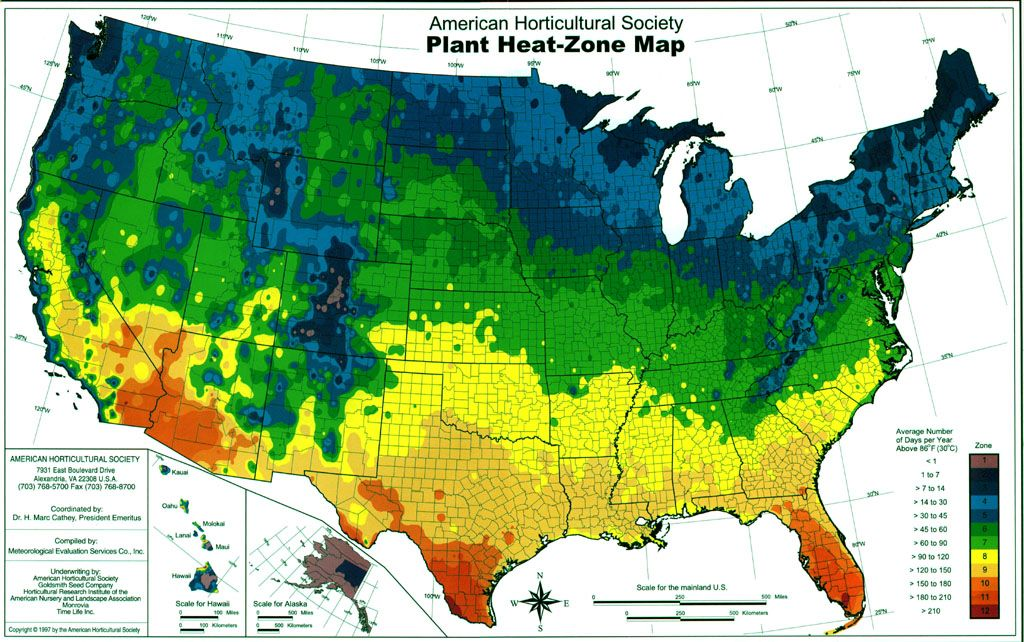
\includegraphics[width=\linewidth]{Heat_Zone_Map_USA.jpg}
	\caption{AHS Heat Zone Map of the US}
	\label{fig:AHS Heat Zone Map}
\end{figure}

\newpage
From these images we can see that there is a more general pattern going on here. 
We have a heat function which is as follows: \\ 
$F : \mathbb{R}^4 \to \mathbb{R}$
Where the inputs to $F$ are $r,\theta,\phi,\tau$ which are: radial distance r, polar angle $\theta$ (theta), azimuthal angle $\phi$ (phi), time $\tau$ (tau). Additionally, the output is the heat at that point in space-time. 
Then when you pick a time, you can project the colored 3D shape onto a 2D image. That wouldn't give you either of the figures below however. Those are calculations, based on the tables, are a way of binning the information to make it easier to understand. 

https://wiki.openstreetmap.org/wiki/Smrender
\href{http://maperitive.net/docs/}{Maperitive} \\
\href{https://wiki.openstreetmap.org/wiki/Rendering}{wiki on map apis}


\end{document}



